\section{Collaborative and Augmentative Systems}


\begin{wrapfigure}{r}{40mm}
  \begin{center}
    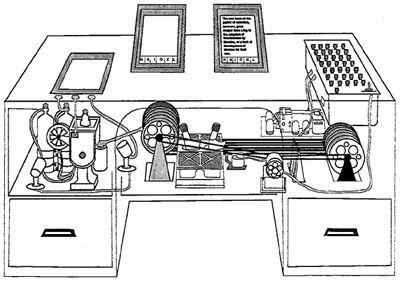
\includegraphics[scale=0.4]{images/memex.jpg}
  \end{center}
  \caption{ Memex, as it was illustrated for LIFE Magazine, 1945. The
    desk contains two main microfilm projectors and mechanical
    apparatus to retrieve the pages for a given
    trail. \cite{hypertext:muller__vision_and_reality}}
\end{wrapfigure}

Users nowadays use several metaphors for networked computers, such as
links, bookmarks, hypertext, web, publishing, collaborative editing
and so forth. These concepts seem ``natural'', but they are as
artificial as the tools that embody them. We can trace their creation
to their modern creator, Vannevar
Bush. \footnote{ Bush as responsible for a great deal more, such as being the man
responsible for the creation of the modern american military-scientific
establishment. \cite{history:pascal__godfather} } Bush, in his highly
influential 1945 article \cite{hypertext:bush__as_we_may_think}
elaborated about the memex, which had a stark similarity with the
modern personal computer and the internet:

\begin{quotation}
  The owner of the memex, let us say, is interested in the origin and
  properties of the bow and arrow. Specifically he is studying why the
  short Turkish bow was apparently superior to the English long bow in
  the skirmishes of the Crusades. He has dozens of possibly pertinent
  books and articles in his memex. First he runs through an
  encyclopedia, finds an interesting but sketchy article, leaves it
  projected. Next, in a history, he finds another pertinent item, and
  ties the two together. Thus he goes, building a trail of many
  items. Occasionally he inserts a comment of his own, either linking
  it into the main trail or joining it by a side trail to a particular
  item. When it becomes evident that the elastic properties of
  available materials had a great deal to do with the bow, he branches
  off on a side trail which takes him through textbooks on elasticity
  and tables of physical constants. He inserts a page of longhand
  analysis of his own. Thus he builds a trail of his interest through
  the maze of materials available to him. 
\end{quotation}


\begin{wrapfigure}{r}{40mm}
  \begin{center}
    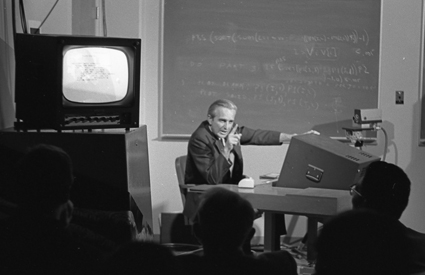
\includegraphics[scale=0.4]{images/engelbart-demo.jpg}
  \end{center}
  \caption{Engelbart demo, 1968.}
\end{wrapfigure}

But if Bush was the original thinker, the original builder was Douglas
Engelbart. His efforts resulted in \emph{Not just hypertext, but
  graphics, multiple panes, efficient navigation and command input,
  interactive collaborative work, etc. An entire conceptual world and
  world view }\cite{smalltalk:kay_alan__early_history_smalltalk}
\cite{intelligence:engelbart__augmenting}.

Engelbart's 1968 demonstration took place in the American Federation of
Information Processing Societies' Fall Joint Computer Conference. It
shook the world then, and it when on the have an enormous amount of
influence in the community that created the personal computer
revolution. \cite{hypertext:muller__vision_and_reality}

\begin{quote}
  The impact of this vision was to produce in the minds of those who
  were ``eager to be augmented'' a compelling metaphor of what
  interactive computing should be like, and I immediately adopted many
  of the ideas for the FLEX machine. 
  \cite{smalltalk:kay_alan__early_history_smalltalk}
\end{quote}
